%
\documentclass[10pt,journal,compsoc]{IEEEtran}
\usepackage{hyperref}
\usepackage{xspace}
\usepackage{algorithm}
\usepackage[noend]{algpseudocode}
\usepackage{amsbsy}
\usepackage{amsthm}
\usepackage{helvet}
\usepackage{enumerate}
\usepackage{amsmath}
\usepackage{amstext}
\usepackage{amsfonts}
\usepackage{graphicx}
\usepackage{multirow}
\usepackage{subfig}
\usepackage{comment}
\usepackage{cases}
\usepackage{xcolor}
\usepackage{epstopdf}
\usepackage[normalem]{ulem}
\usepackage{diagbox}

\newtheorem{Algorithm}{Algorithm}[section]
\newtheorem{Definition}{Definition}[section]
\newtheorem{Example}{Example}[section]
\newtheorem{Proposition}{Proposition}[section]
\newtheorem{Lemma}{Lemma}[section]
\newtheorem{Theorem}{Theorem}[section]
\newtheorem{Proof}{Proof}[section]
\newtheorem{Corollary}{Corollary}[section]
\newtheorem{Conjecture}{Conjecture}[section]
\newtheorem{Problem}{Problem}[section]
\newtheorem{Notation}{Notation}[section]
\newtheorem{Setup}{Problem Setup}[section]

\ifCLASSOPTIONcompsoc
  % The IEEE Computer Society needs nocompress option
  % requires cite.sty v4.0 or later (November 2003)
  \usepackage[nocompress]{cite}
\else
  % normal IEEE
  \usepackage{cite}
\fi

\newcommand\MYhyperrefoptions{bookmarks=true,bookmarksnumbered=true,
pdfpagemode={UseOutlines},plainpages=false,pdfpagelabels=true,
colorlinks=true,linkcolor={black},citecolor={black},urlcolor={black},
pdftitle={Bare Demo of IEEEtran.cls for Computer Society Journals},%<!CHANGE!
pdfsubject={Typesetting},%<!CHANGE!
pdfauthor={Michael D. Shell},%<!CHANGE!
pdfkeywords={Computer Society, IEEEtran, journal, LaTeX, paper,
             template}}%<^!CHANGE!

\hyphenation{op-tical net-works semi-conduc-tor}

\begin{document}

\title{Conformal Equivalence}

\author{Vikas Rao\\
U1072596\\
vikas.k.rao@utah.edu\\
Electrical \& Computer Engineering, University of Utah\\
}

% The paper headers
\markboth{ECE-6750 Project Report}%
{Shell \MakeLowercase{\textit{et al.}}: Bare Advanced Demo of IEEEtran.cls for IEEE Computer Society Journals}

\IEEEtitleabstractindextext{%
\begin{abstract}
Designing a specification and making sure the protocol never leads to a deadlock while achieving its intended function cannot be verified by simulation alone.  Even by some means if we do exhaustive simulation, it doesn’t guarantee a complete coverage of the state space and needs a formal approach to verify specification under all permissible delay behaviors. This problem is extensive in asynchronous designs, as a hazard might manifest into a failure under a very particular set of delays.
Given a circuit implementation of this specification, we need to verify that this circuit is hazard free under all permissible delay behaviors as well. The system verification challenge is then to verify that this circuit conforms to the specification in terms of functional implementation. Given this problem statement, the goal of the project is to derive a receptive state graph for the circuit and verify if all possible behaviors of circuit are allowed behaviors in specification.

\end{abstract}

% Note that keywords are not normally used for peerreview papers.
\begin{IEEEkeywords}
Verification, State Graph, Petri-Net.
\end{IEEEkeywords}}


% make the title area
\maketitle

\IEEEdisplaynontitleabstractindextext
% \IEEEdisplaynontitleabstractindextext has no effect when using
% compsoc under a non-conference mode.


% For peer review papers, you can put extra information on the cover
% page as needed:
% \ifCLASSOPTIONpeerreview
% \begin{center} \bfseries EDICS Category: 3-BBND \end{center}
% \fi
%
% For peerreview papers, this IEEEtran command inserts a page break and
% creates the second title. It will be ignored for other modes.
\IEEEpeerreviewmaketitle

\IEEEraisesectionheading{\section{Introduction}\label{sec:introduction}}

Conformal equivalence is the process of verifying whether a circuit conforms to the specification. The goal here is to make sure that a protocol, circuit has all the desired properties and is hazard free. We need to make sure protocol never deadlocks and acknowledges a request in bounded amount of time. For a circuit with $n$-bit input, exhaustive simulation requires $2^n$ vectors to verify functionality, which is impractical for large designs. Despite exhaustive simulation, completeness of the design is not guaranteed. Especially in asynchronous design, the hazard manifests only under a very particular set of delays. Verification needs to make sure all permissible delay behaviors are modeled and that the circuit operates correctly under all the delay combinations.
Then the system level verification challenge is to verify that all circuit behaviors are allowed by a given specification.

\section{Scope and Objective}

The goal of the project is to implement an algorithm to build a receptive State Graph(SG) which can model and verify the circuit under all permissible delay models. The algorithm will build the SG from a Labeled Petri-Net(LPN) format which is the specification. The specification is given in a file(*.lpn) describing the petri-net transitions for the input and output excitations. To model the circuit gate behavior, the circuit implementation structure file (*.prs) is read, wherein the gates of the circuit are described for every output excitation(rise/fall) and their relation to input excitations. For every gate in the design, we will model a cube which comprises of all the variables from the circuit packed into a vector. For every cube in the circuit, the inclusive states are identified from the SG and all the unexpected output transitions which lead to failure state are modeled. The SG is then pruned to remove transitions which are unlikely to happen. The system verification goal is then to verify if all the individual gate behaviors of the circuit are allowed behaviors in the state graph implemented for specification. 

\section{Preliminaries}

\subsection{Labeled Petri-nets}
A Petri-net is a bipartite digraph where the vertex set is partitioned into set of places($P$) and transitions($T$). The set of arcs($F$) is composed of pairs where one element is from $P$ and the other is from $T$. A Marking $M$, for a Petri-net is a function that maps places to natural numbers. 

\begin{align*}
F \subseteq (P \times T) \cup (T \times P) \\
M : P \rightarrow N
\end{align*}

A Petri-net is defined as in the tuple below, where $M_0$ is the initial marking. 
\begin{align*}
\langle P,T,F,M_0 \rangle
\end{align*}

A C-element and its Labeled Petri-net is as shown in the figure~\ref{celem_lpn}. 

\subsection{State Graphs}
To use a Petri-net to model circuits, we must relate the transitions to events on signal wires.
One such modeling is a \textit{Signal Transition Graph}(STG) which is a labeled Safe Petri-net 
described using the tuple - 

\begin{align*}
\langle P,T,F,M_0,N,s_0,\lambda_T\rangle
\end{align*}  

where: $N=I\cup O$ is the set of Input and output signals, $s_0$ is the initial state and $\lambda_T = T \rightarrow N \times \{+,-\}$ 
is the transition labeling function. Each transition is labeled with either a rising transition($+$) or falling transition($-$).
A circuit can be modeled from a given STG if we can find the State Graph(SG) for the same. The SG is modeled by the tuple -

\begin{align*}
\langle S, \delta, \lambda_S \rangle
\end{align*}   

\begin{figure}[hbt]
  \begin{center}
  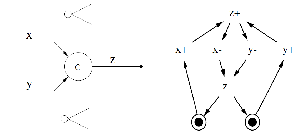
\includegraphics[scale = 0.28]{celem_lpn}
  \end{center}
  \vspace{-2ex}
  \caption{circuit and LPN for a C-element}
  \label{celem_lpn}
  \vspace{-1ex}
\end{figure}

where: $S$ is the set of states, $\delta \subseteq S \times T \times S$ is the set of transitions, and $\lambda_S: S \rightarrow (N \rightarrow \{0,1\})$ is the
state labeling function. Each state $S$ is labeled with a vector $\langle s(0),s(1)...s(n)\rangle$ where $s(i)$ is $0,1,R,F$ indicating value returned by $\lambda_S$. 

For each state, we can determine the value that each signal is tending to. For a state $s_i$, there exists a transition on signal $u_i$ to $s_j$, which excites the signal $u_i$.
\begin{align*}
\exists(s_i,t,s_j)\in \delta\cdot\lambda_T(t) = u_i + \forall \lambda_T(t)= u_i-
\end{align*}

If there exists no such transition, then $u_i$ is said to be in equilibrium.
The value each signal is tending to in any state is called its implied value.
If the signal is excited, the implied value of $u_i$ is $\bar{s_i}$, else if the signal is in equilibrium, then the implied value is $s_i$
The implied state, $s'$ is labeled with a binary vector $\langle s'(0),s'(1)\dots s'(n)\rangle$ of the implied values.
The function $X : S \rightarrow 2^N$ returns the set of excited signals in a given state defined as-
\begin{align*}
 X(s) = {u_i \in S | s(i) \neq s'(i)}
\end{align*}\\
The next state transitions are defined based on the function $X(s)$.\\
When $u_i \in X(s)$ and $s(i) = 0, s(i)$ in SG is marked with “R”.\\
When $u_i \in X(s)$ and $s(i) = 1, s(i)$ in SG is marked with “F”.

\begin{figure}[hbt]
  \begin{center}
  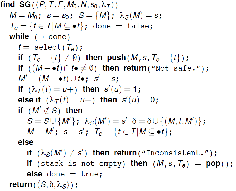
\includegraphics[scale = 0.37]{sg_algo}
  \end{center}
  \vspace{-2ex}
  \caption{State Graph algorithm}
  \label{sg_algo}
  \vspace{-1ex}
\end{figure}

The algorithm to find the SG from a given STG(LPN) is as shown in figure~\ref{sg_algo}.
Any SG is said to be well-formed if for each state transition $(s_i,t,s_j) \in \delta$, exactly
one signal changes value and its value is consistent with the transition. The property is defined as \textit{consistent state assignment}, and a SG is said to be consistent if

\begin{align*}
\forall (s_i,t,s_j) \in \delta.\forall u \in N .(\lambda_T(t) \neq u* \wedge s_i(u) = s_j(u))\\ \vee
(\lambda_T(t) = u+ \wedge s_i(u) = 0 \wedge s_j(u) = 1) \\ \vee (\lambda_T(t) \neq u- \wedge s_i(u)= 1 \wedge s_j(u)= 1)
\end{align*} 
where $*$ represents either $+$ or $-$.

The SG also has a \textit{Unique State Assignment} which requires that no two different states have identical values for the vector signals.

\begin{align*}
\forall s_i,s_j \in S: s_i\neq s_j.\lambda(s_i) \neq \lambda(s_j)
\end{align*} 

To verify the behavior of circuit against the allowed behaviors from specification, we need to model a receptive state graph, meaning the state of a circuit should not prevent an 
input from happening -
\begin{align*}
PI\subseteq P
\end{align*}
Where: $P=S\cup F$: $S$ is the set of all successful sequence of signal changes and $F$ is the set of all failure sequences.
The receptive State Graph for the generalized C-element is as shown in the figure~\ref{celem_sg}. 

\begin{figure}[hbt]
  \begin{center}
  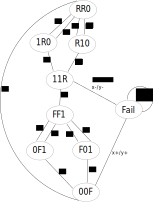
\includegraphics[scale = 0.45]{celem_sg}
  \end{center}
  \vspace{-2ex}
  \caption{Receptive State Graph for the C-element}
  \label{celem_sg}
  \vspace{-1ex}
\end{figure}


\section{Implementation}
The overall high level approach is as mentioned in algorithm~\ref{algo:confequ}. The actual conformal checking requires deriving receptive SG's from both circuit and the specification and compare each state to incrementally prune the edges and redirecting illegal transitions to $Fail$ state. For a $n$-bit wide state vector, we could have also derived a full blown state graph with $2^n$ states and $2^n$ edges to/from each state. Owing to delayed start, the current implementation will build a reduced State Graph from the LPN to start with and then visit every gate cube's inclusive states and prune the edges accordingly and check for fail transitions. In-turn verify that at all nodes, all transitions where the specification is failure-free, the circuit
is also failure-free. 

\subsection{Circuit Cubes and State Graph}
To extract the behavior from the circuit gates, we will form cubes which represent each excitation output. For every circuit, all the variables will be packed into a cube vector packet. For every output excitation, the vector cube is represented based on the following notation: `1' if the literal is in the its trigger, `0' if the literal is in its negated form, `-' if it is absent.
Given below is a sample circuit file with gate excitations and their respective cubes.

Cube vector - $\langle x,y,z \rangle$
\begin{itemize}
\item$[+x: (\neg y \& \neg z)]$ - Set Cube:[- 0 0]\\ 
\item$[-x: (z)]$ - Reset Cube:[- - 1] \\
\item$[ y: (z)]$ Combinational \\
\item$[ y: (x)]$ Combinational: Set Cube:[[- - 1],[1 - -]] 
\end{itemize}

\begin{algorithm}
\caption{conformal Equivalence}
\label{algo:confequ}
\begin{algorithmic}[1]

\Procedure{$circuit\_verification\_algo$}{\$FILE1,\$FILE2} 
// FILE1 = Circuit(*.prs), FILE2 = Spec(*.lpn)
\State $hash\_cubes = find\_cubes(\$FILE1)$
\State $hash\_SG = find\_sg(\$FILE2)$
\For {$\text{each cube in hash\_cubes}$}
\For {$\text{inclusive states from hash\_SG}$}
\State {$\rightarrow\text{Redirect illegal transitions to 'Fail' State}$}
\State {$\rightarrow\text{Prune transitions which are not allowed}$}
\EndFor
\EndFor 
\EndProcedure
\end{algorithmic}
\end{algorithm}

A generalized C-element is expressed as Set and Reset cubes for it's rising transition($+$) and falling transition($+$) respectively($-$). A combinational logic is expressed as a list of Set cubes only while the reset cubes are ignored. The structure is stored in a HashTable data structure with keys as the output excitation signals and cubes as the list of values. 

The algorithm to find SG is as mentioned in the figure~\ref{sg_algo}. 
From the given LPN, the initial state($s_0$), Markings($M_0$), and transitions($T$) are read and a SG is derived. 
The actual verification follows that a State Graph be derived for every individual gate transition and a final composite SG is derived and checked against Specification SG for fail states.
But since there is no initial state defined for gC gate descriptions, deriving a SG from the circuit is cumbersome. Also it requires that we traverse individual gate SG's and modify all graphs to finally arrive at a composite SG.
The composite graph is built by pruning
the state space and transitions based on the behavior described by the individual gates in the circuit.

The State Graph is also stored in a HashTable data structure where the state vector names are the keys and the values are edges marked as a object derived from links describing the transitions causing them and next state functions.

\subsection{Redirecting/Pruning edges}
Once we are available with the cubes describing the individual gates of the circuit and a State Graph from the LPN specification, we will check for state inclusion, and prune the graph.
Every node in state graph which is implicitly covered by gate cubes needs to be checked for fail state. Any unexpected outputs and disabling
will lead to fail state. The following are some of the rules between current state and next state which will be followed for pruning and redirecting the edges.

\begin{itemize}
\item A transition is success in composite graph state node, if it is a success in every individual
gate transition. 
\item A transition is a failure in composite graph, if it is a failure in any of the individual gate transition.
\item A Fail state occurs when an input transitions occur at the wrong time.
\item A rising output transition($R$) cannot change to zero($0$) in consecutive state (should be redirected to Fail
sate).
\item A falling output transition($F$) cannot change to one($1$) in consecutive state (should be redirected to Fail
sate).
\item For a Set cube, the falling output transition($-$) from every implicit state node satisfying the
\item For a Reset cube, the rising output transition($+$) from every implicit state node satisfying the
state inclusion should be discarded.
\end{itemize}

\subsection{Progress}
As of now, the extraction of cubes from the circuit is completed, and the code for SG building has some issues and I am working on fixing it. The final intent 
of the project is to implement the algorithm~\ref{algo:confequ} completely and test a set of examples from reference ~\cite{IEEEhowto:cjmyers}, and as well as from the ATACS repo, discuss and analyze the outcome.

\begin{thebibliography}{1}

\bibitem{IEEEhowto:cjmyers}
C. J. Myers, \emph{{A}synchronous {C}ircuit {D}esign}, John Wiley and Sons, Jul 1, 2001.

\end{thebibliography}

% that's all folks
\end{document}


